
%% bare_conf.tex
%% V1.3
%% 2007/01/11
%% by Michael Shell
%% See:
%% http://www.michaelshell.org/
%% for current contact information.
%%
%% This is a skeleton file demonstrating the use of IEEEtran.cls
%% (requires IEEEtran.cls version 1.7 or later) with an IEEE conference paper.
%%
%% Support sites:
%% http://www.michaelshell.org/tex/ieeetran/
%% http://www.ctan.org/tex-archive/macros/latex/contrib/IEEEtran/
%% and
%% http://www.ieee.org/

%%*************************************************************************
%% Legal Notice:
%% This code is offered as-is without any warranty either expressed or
%% implied; without even the implied warranty of MERCHANTABILITY or
%% FITNESS FOR A PARTICULAR PURPOSE!
%% User assumes all risk.
%% In no event shall IEEE or any contributor to this code be liable for
%% any damages or losses, including, but not limited to, incidental,
%% consequential, or any other damages, resulting from the use or misuse
%% of any information contained here.
%%
%% All comments are the opinions of their respective authors and are not
%% necessarily endorsed by the IEEE.
%%
%% This work is distributed under the LaTeX Project Public License (LPPL)
%% ( http://www.latex-project.org/ ) version 1.3, and may be freely used,
%% distributed and modified. A copy of the LPPL, version 1.3, is included
%% in the base LaTeX documentation of all distributions of LaTeX released
%% 2003/12/01 or later.
%% Retain all contribution notices and credits.
%% ** Modified files should be clearly indicated as such, including  **
%% ** renaming them and changing author support contact information. **
%%
%% File list of work: IEEEtran.cls, IEEEtran_HOWTO.pdf, bare_adv.tex,
%%                    bare_conf.tex, bare_jrnl.tex, bare_jrnl_compsoc.tex
%%*************************************************************************

% *** Authors should verify (and, if needed, correct) their LaTeX system  ***
% *** with the testflow diagnostic prior to trusting their LaTeX platform ***
% *** with production work. IEEE's font choices can trigger bugs that do  ***
% *** not appear when using other class files.                            ***
% The testflow support page is at:
% http://www.michaelshell.org/tex/testflow/



% Note that the a4paper option is mainly intended so that authors in
% countries using A4 can easily print to A4 and see how their papers will
% look in print - the typesetting of the document will not typically be
% affected with changes in paper size (but the bottom and side margins will).
% Use the testflow package mentioned above to verify correct handling of
% both paper sizes by the user's LaTeX system.
%
% Also note that the "draftcls" or "draftclsnofoot", not "draft", option
% should be used if it is desired that the figures are to be displayed in
% draft mode.
%
\documentclass[conference]{IEEEtran}
% Add the compsoc option for Computer Society conferences.
%
% If IEEEtran.cls has not been installed into the LaTeX system files,
% manually specify the path to it like:
% \documentclass[conference]{../sty/IEEEtran}





% Some very useful LaTeX packages include:
% (uncomment the ones you want to load)


% *** MISC UTILITY PACKAGES ***
%
%\usepackage{ifpdf}
% Heiko Oberdiek's ifpdf.sty is very useful if you need conditional
% compilation based on whether the output is pdf or dvi.
% usage:
% \ifpdf
%   % pdf code
% \else
%   % dvi code
% \fi
% The latest version of ifpdf.sty can be obtained from:
% http://www.ctan.org/tex-archive/macros/latex/contrib/oberdiek/
% Also, note that IEEEtran.cls V1.7 and later provides a builtin
% \ifCLASSINFOpdf conditional that works the same way.
% When switching from latex to pdflatex and vice-versa, the compiler may
% have to be run twice to clear warning/error messages.






% *** CITATION PACKAGES ***
%
\usepackage{cite}
% cite.sty was written by Donald Arseneau
% V1.6 and later of IEEEtran pre-defines the format of the cite.sty package
% \cite{} output to follow that of IEEE. Loading the cite package will
% result in citation numbers being automatically sorted and properly
% "compressed/ranged". e.g., [1], [9], [2], [7], [5], [6] without using
% cite.sty will become [1], [2], [5]--[7], [9] using cite.sty. cite.sty's
% \cite will automatically add leading space, if needed. Use cite.sty's
% noadjust option (cite.sty V3.8 and later) if you want to turn this off.
% cite.sty is already installed on most LaTeX systems. Be sure and use
% version 4.0 (2003-05-27) and later if using hyperref.sty. cite.sty does
% not currently provide for hyperlinked citations.
% The latest version can be obtained at:
% http://www.ctan.org/tex-archive/macros/latex/contrib/cite/
% The documentation is contained in the cite.sty file itself.






% *** GRAPHICS RELATED PACKAGES ***
%
\ifCLASSINFOpdf
  \usepackage[pdftex]{graphicx}
  \usepackage{epstopdf}
  % declare the path(s) where your graphic files are
  \graphicspath{{E:/Documents/Iowa_State/2013-2014/COMS583/FinalProject/}}
  % and their extensions so you won't have to specify these with
  % every instance of \includegraphics
  \DeclareGraphicsExtensions{.pdf,.jpeg,.png}
\else
  % or other class option (dvipsone, dvipdf, if not using dvips). graphicx
  % will default to the driver specified in the system graphics.cfg if no
  % driver is specified.
  % \usepackage[dvips]{graphicx}
  % declare the path(s) where your graphic files are
  % \graphicspath{{../eps/}}
  % and their extensions so you won't have to specify these with
  % every instance of \includegraphics
  % \DeclareGraphicsExtensions{.eps}
\fi
% graphicx was written by David Carlisle and Sebastian Rahtz. It is
% required if you want graphics, photos, etc. graphicx.sty is already
% installed on most LaTeX systems. The latest version and documentation can
% be obtained at:
% http://www.ctan.org/tex-archive/macros/latex/required/graphics/
% Another good source of documentation is "Using Imported Graphics in
% LaTeX2e" by Keith Reckdahl which can be found as epslatex.ps or
% epslatex.pdf at: http://www.ctan.org/tex-archive/info/
%
% latex, and pdflatex in dvi mode, support graphics in encapsulated
% postscript (.eps) format. pdflatex in pdf mode supports graphics
% in .pdf, .jpeg, .png and .mps (metapost) formats. Users should ensure
% that all non-photo figures use a vector format (.eps, .pdf, .mps) and
% not a bitmapped formats (.jpeg, .png). IEEE frowns on bitmapped formats
% which can result in "jaggedy"/blurry rendering of lines and letters as
% well as large increases in file sizes.
%
% You can find documentation about the pdfTeX application at:
% http://www.tug.org/applications/pdftex





% *** MATH PACKAGES ***
%
%\usepackage[cmex10]{amsmath}
% A popular package from the American Mathematical Society that provides
% many useful and powerful commands for dealing with mathematics. If using
% it, be sure to load this package with the cmex10 option to ensure that
% only type 1 fonts will utilized at all point sizes. Without this option,
% it is possible that some math symbols, particularly those within
% footnotes, will be rendered in bitmap form which will result in a
% document that can not be IEEE Xplore compliant!
%
% Also, note that the amsmath package sets \interdisplaylinepenalty to 10000
% thus preventing page breaks from occurring within multiline equations. Use:
%\interdisplaylinepenalty=2500
% after loading amsmath to restore such page breaks as IEEEtran.cls normally
% does. amsmath.sty is already installed on most LaTeX systems. The latest
% version and documentation can be obtained at:
% http://www.ctan.org/tex-archive/macros/latex/required/amslatex/math/





% *** SPECIALIZED LIST PACKAGES ***
%
%\usepackage{algorithmic}
% algorithmic.sty was written by Peter Williams and Rogerio Brito.
% This package provides an algorithmic environment fo describing algorithms.
% You can use the algorithmic environment in-text or within a figure
% environment to provide for a floating algorithm. Do NOT use the algorithm
% floating environment provided by algorithm.sty (by the same authors) or
% algorithm2e.sty (by Christophe Fiorio) as IEEE does not use dedicated
% algorithm float types and packages that provide these will not provide
% correct IEEE style captions. The latest version and documentation of
% algorithmic.sty can be obtained at:
% http://www.ctan.org/tex-archive/macros/latex/contrib/algorithms/
% There is also a support site at:
% http://algorithms.berlios.de/index.html
% Also of interest may be the (relatively newer and more customizable)
% algorithmicx.sty package by Szasz Janos:
% http://www.ctan.org/tex-archive/macros/latex/contrib/algorithmicx/




% *** ALIGNMENT PACKAGES ***
%
%\usepackage{array}
% Frank Mittelbach's and David Carlisle's array.sty patches and improves
% the standard LaTeX2e array and tabular environments to provide better
% appearance and additional user controls. As the default LaTeX2e table
% generation code is lacking to the point of almost being broken with
% respect to the quality of the end results, all users are strongly
% advised to use an enhanced (at the very least that provided by array.sty)
% set of table tools. array.sty is already installed on most systems. The
% latest version and documentation can be obtained at:
% http://www.ctan.org/tex-archive/macros/latex/required/tools/


%\usepackage{mdwmath}
%\usepackage{mdwtab}
% Also highly recommended is Mark Wooding's extremely powerful MDW tools,
% especially mdwmath.sty and mdwtab.sty which are used to format equations
% and tables, respectively. The MDWtools set is already installed on most
% LaTeX systems. The lastest version and documentation is available at:
% http://www.ctan.org/tex-archive/macros/latex/contrib/mdwtools/


% IEEEtran contains the IEEEeqnarray family of commands that can be used to
% generate multiline equations as well as matrices, tables, etc., of high
% quality.


%\usepackage{eqparbox}
% Also of notable interest is Scott Pakin's eqparbox package for creating
% (automatically sized) equal width boxes - aka "natural width parboxes".
% Available at:
% http://www.ctan.org/tex-archive/macros/latex/contrib/eqparbox/





% *** SUBFIGURE PACKAGES ***
%\usepackage[tight,footnotesize]{subfigure}
% subfigure.sty was written by Steven Douglas Cochran. This package makes it
% easy to put subfigures in your figures. e.g., "Figure 1a and 1b". For IEEE
% work, it is a good idea to load it with the tight package option to reduce
% the amount of white space around the subfigures. subfigure.sty is already
% installed on most LaTeX systems. The latest version and documentation can
% be obtained at:
% http://www.ctan.org/tex-archive/obsolete/macros/latex/contrib/subfigure/
% subfigure.sty has been superceeded by subfig.sty.



%\usepackage[caption=false]{caption}
%\usepackage[font=footnotesize]{subfig}
% subfig.sty, also written by Steven Douglas Cochran, is the modern
% replacement for subfigure.sty. However, subfig.sty requires and
% automatically loads Axel Sommerfeldt's caption.sty which will override
% IEEEtran.cls handling of captions and this will result in nonIEEE style
% figure/table captions. To prevent this problem, be sure and preload
% caption.sty with its "caption=false" package option. This is will preserve
% IEEEtran.cls handing of captions. Version 1.3 (2005/06/28) and later
% (recommended due to many improvements over 1.2) of subfig.sty supports
% the caption=false option directly:
%\usepackage[caption=false,font=footnotesize]{subfig}
%
% The latest version and documentation can be obtained at:
% http://www.ctan.org/tex-archive/macros/latex/contrib/subfig/
% The latest version and documentation of caption.sty can be obtained at:
% http://www.ctan.org/tex-archive/macros/latex/contrib/caption/




% *** FLOAT PACKAGES ***
%
%\usepackage{fixltx2e}
% fixltx2e, the successor to the earlier fix2col.sty, was written by
% Frank Mittelbach and David Carlisle. This package corrects a few problems
% in the LaTeX2e kernel, the most notable of which is that in current
% LaTeX2e releases, the ordering of single and double column floats is not
% guaranteed to be preserved. Thus, an unpatched LaTeX2e can allow a
% single column figure to be placed prior to an earlier double column
% figure. The latest version and documentation can be found at:
% http://www.ctan.org/tex-archive/macros/latex/base/



%\usepackage{stfloats}
% stfloats.sty was written by Sigitas Tolusis. This package gives LaTeX2e
% the ability to do double column floats at the bottom of the page as well
% as the top. (e.g., "\begin{figure*}[!b]" is not normally possible in
% LaTeX2e). It also provides a command:
%\fnbelowfloat
% to enable the placement of footnotes below bottom floats (the standard
% LaTeX2e kernel puts them above bottom floats). This is an invasive package
% which rewrites many portions of the LaTeX2e float routines. It may not work
% with other packages that modify the LaTeX2e float routines. The latest
% version and documentation can be obtained at:
% http://www.ctan.org/tex-archive/macros/latex/contrib/sttools/
% Documentation is contained in the stfloats.sty comments as well as in the
% presfull.pdf file. Do not use the stfloats baselinefloat ability as IEEE
% does not allow \baselineskip to stretch. Authors submitting work to the
% IEEE should note that IEEE rarely uses double column equations and
% that authors should try to avoid such use. Do not be tempted to use the
% cuted.sty or midfloat.sty packages (also by Sigitas Tolusis) as IEEE does
% not format its papers in such ways.





% *** PDF, URL AND HYPERLINK PACKAGES ***
%
%\usepackage{url}
% url.sty was written by Donald Arseneau. It provides better support for
% handling and breaking URLs. url.sty is already installed on most LaTeX
% systems. The latest version can be obtained at:
% http://www.ctan.org/tex-archive/macros/latex/contrib/misc/
% Read the url.sty source comments for usage information. Basically,
% \url{my_url_here}.





% *** Do not adjust lengths that control margins, column widths, etc. ***
% *** Do not use packages that alter fonts (such as pslatex).         ***
% There should be no need to do such things with IEEEtran.cls V1.6 and later.
% (Unless specifically asked to do so by the journal or conference you plan
% to submit to, of course. )
% correct bad hyphenation here

\usepackage{tikz}


\begin{document}
%
% paper title
% can use linebreaks \\ within to get better formatting as desired
\title{Break Out: Implementing Old School Games on FPGAs}


% author names and affiliations
% use a multiple column layout for up to three different
% affiliations
\author{\IEEEauthorblockN{Brian Nakayama}
\IEEEauthorblockA{Department of Computer Science\\
Iowa State University\\
Ames, Iowa 50011}
\and
\IEEEauthorblockN{Mahieddine Dellabani}
\IEEEauthorblockA{Ensimag, School of Computer Engineering\\
Grenoble INP\\
Grenoble, France}}

% conference papers do not typically use \thanks and this command
% is locked out in conference mode. If really needed, such as for
% the acknowledgment of grants, issue a \IEEEoverridecommandlockouts
% after \documentclass

% for over three affiliations, or if they all won't fit within the width
% of the page, use this alternative format:
%
%\author{\IEEEauthorblockN{Michael Shell\IEEEauthorrefmark{1},
%Homer Simpson\IEEEauthorrefmark{2},
%James Kirk\IEEEauthorrefmark{3},
%Montgomery Scott\IEEEauthorrefmark{3} and
%Eldon Tyrell\IEEEauthorrefmark{4}}
%\IEEEauthorblockA{\IEEEauthorrefmark{1}School of Electrical and Computer Engineering\\
%Georgia Institute of Technology,
%Atlanta, Georgia 30332--0250\\ Email: see http://www.michaelshell.org/contact.html}
%\IEEEauthorblockA{\IEEEauthorrefmark{2}Twentieth Century Fox, Springfield, USA\\
%Email: homer@thesimpsons.com}
%\IEEEauthorblockA{\IEEEauthorrefmark{3}Starfleet Academy, San Francisco, California 96678-2391\\
%Telephone: (800) 555--1212, Fax: (888) 555--1212}
%\IEEEauthorblockA{\IEEEauthorrefmark{4}Tyrell Inc., 123 Replicant Street, Los Angeles, California 90210--4321}}




% use for special paper notices
%\IEEEspecialpapernotice{(Invited Paper)}




% make the title area
\maketitle


\begin{abstract}
%\boldmath
Implementing \emph{Breakout} on an FPGA requires design elements found commonly in integrated circuits such as finite state machines and interesting examples of dataflow. As mentioned in the proposal, \emph{Breakout} was originally implemented completely in digital hardware (with no processor or program). In our implementation, we broke down the game into three main modules: the keyboard, the game logic, and the VGA/screen. We further divided these modules into finer grained modules for both modularity and clarity. Though we have not completed an online tutorial for \emph{Breakout} (as we fcused on in our proposal), this document which specifies how our implementation works contains the beginnings of an eventually completed online lesson.
\end{abstract}
% IEEEtran.cls defaults to using nonbold math in the Abstract.
% This preserves the distinction between vectors and scalars. However,
% if the conference you are submitting to favors bold math in the abstract,
% then you can use LaTeX's standard command \boldmath at the very start
% of the abstract to achieve this. Many IEEE journals/conferences frown on
% math in the abstract anyway.

% no keywords




% For peer review papers, you can put extra information on the cover
% page as needed:
% \ifCLASSOPTIONpeerreview
% \begin{center} \bfseries EDICS Category: 3-BBND \end{center}
% \fi
%
% For peerreview papers, this IEEEtran command inserts a page break and
% creates the second title. It will be ignored for other modes.
\IEEEpeerreviewmaketitle



\section{Introduction}We have divided our guide to implementation into three sections comprising of the keyboard controller, the game logic, and the VGA controller. Followed we have provided a list of open issues and lessons learned from our implementation of \emph{Breakout}, as well as possible plans for the future.

\section{Keyboard Controller}










\subsection{Inputs and Outputs}
The inputs for the controller are:
\begin{itemize}
  \item PS2D
  \item PS2C
\end{itemize}

The outputs for the controller are:
\begin{itemize}
  \item scan\_ready
  \item scan\_code
\end{itemize}

\begin{figure*}[!t]
\centering
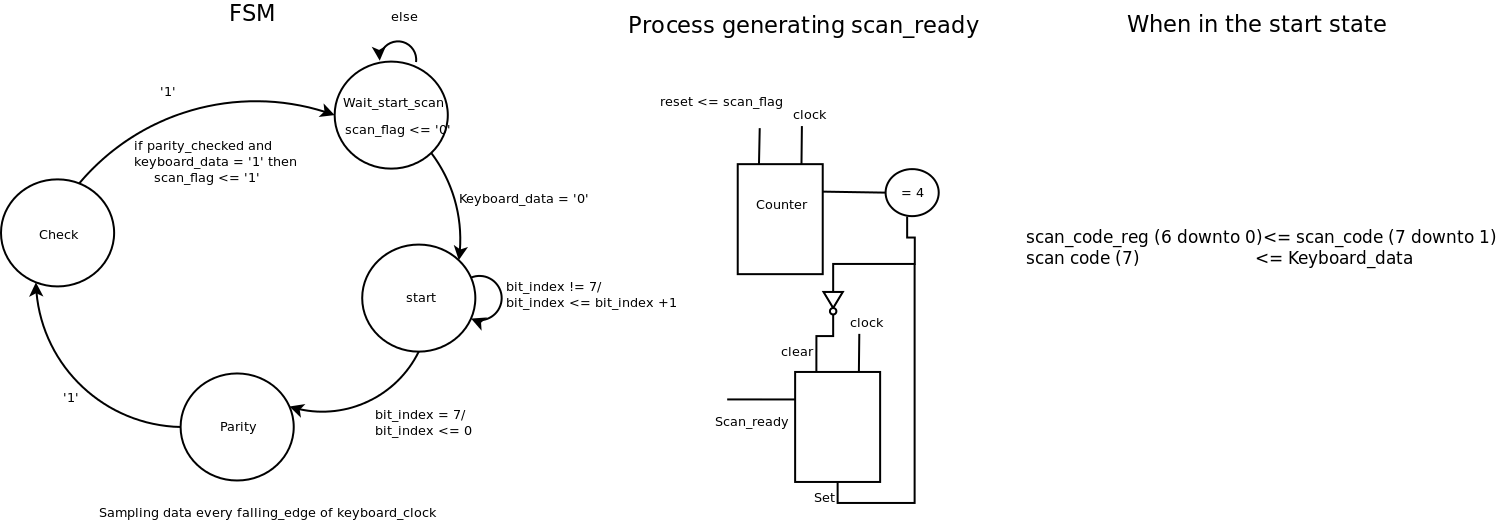
\includegraphics[width=7in]{KBD1}
\caption{The FSM and logic diagram for the keyboard}
\label{KBD1}
\end{figure*}


\begin{figure*}[!t]
\centering
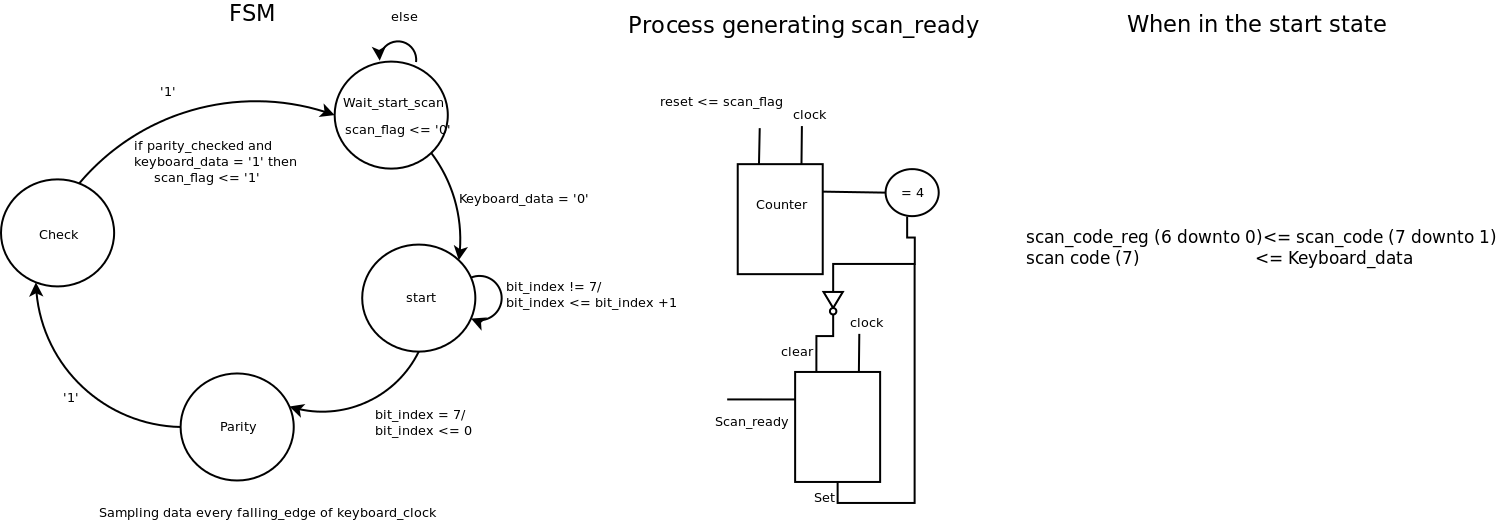
\includegraphics[width=7in]{KBD1}
\caption{The FSM and logic diagram for the keyboard}
\label{KBD1}
\end{figure*}


\begin{figure*}[!t]
\centering
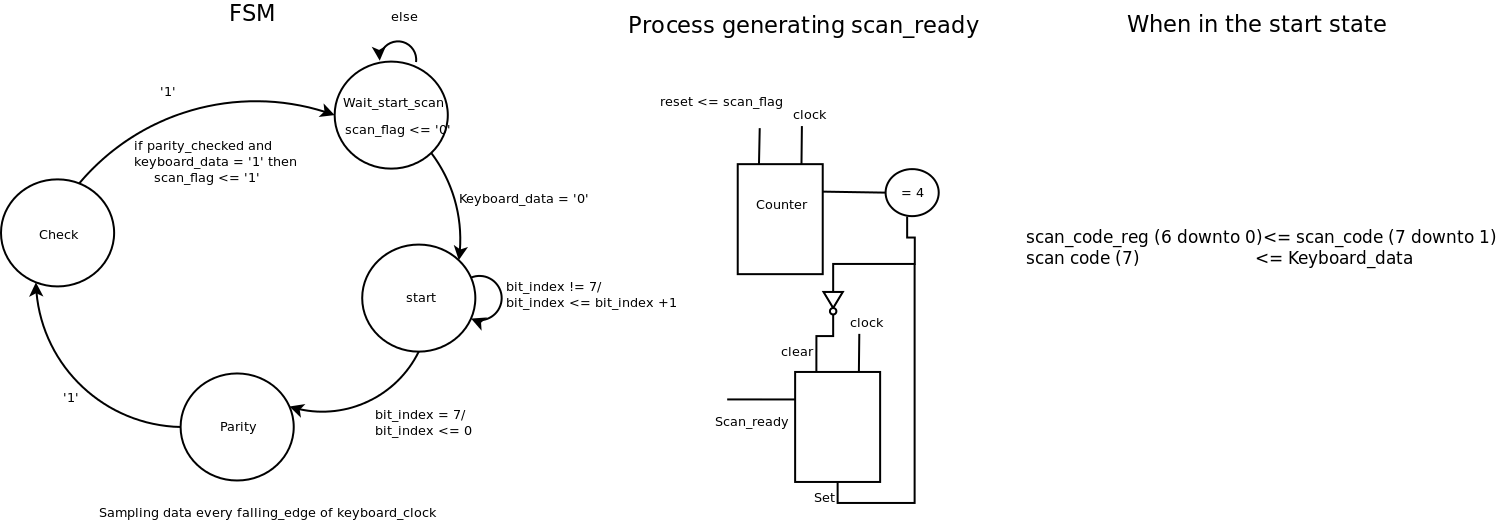
\includegraphics[width=7in]{KBD1}
\caption{The FSM and logic diagram for the keyboard}
\label{KBD1}
\end{figure*}
 
\subsection{The Keyboard}
For the communication between the keyboard and the FPGA board,

the keyboard module (Kbd.vhd) implements a Device to host communication.

Data sent from the keyboard has a 11-bits format: a start bit, 7 bits of data,

a parity bit and a stop bit.



The start and stop bits are always equal to 0 and 1 respectively and the parity bit

corresponds to an odd parity. It means that it is set if there is an even number of one's

in the data bits otherwise it is cleared. This is used for errors checking, so when an

error occures the bit packet is withdrawn.



The 8 bits data correspond to either the scancode of the key pressed, the

key up code (``F0'') or the extend scancode for the extrended keys (``E0''). (see more about it

in the controller section)



The keyboard writes the data bit per bit on the data line (PS2D) when clock(PS2C) is high,

so they can be read by the host when the clock is low.



During the sampling, the 8 bits data are gathered into a 1-byte vector using

the following shifting operation:



1-  scan_code_reg (6 downto 0) <= scan_code_reg (7 downto 1);

2-  scan_code_reg (7)          <= keyboard_data;



The new incoming keyboard_data bit is always received in the 7th index after shifting the previous bits

to the right.



when data are ready, the signal scan_ready is set to one for one clock cycle notifying thus

the controller. Figure n°? (b) shows how the scan_ready is either set or cleared.



Figure n°? (a) displays a high level view of the device to host communication.


\subsection{The Controller}

inputs: scan_ready scan_code outputs: control_en, control_mode, control_signal



The keyboard uses scan codes to communicate the key pressed data. Each key has a particular

scan code (1 byte). If a key is pressed, its scan code is sent and if it's held down, the scan

code will be sent repeatedly once every 100ms(refer to DATAsheet). When released, the keyboard

send the key-up code (``F0'') followed by the scan code of the realesed key.



However there are special keys in the kyeboard, where the byte ``E0'' is sent first ahead of the scan

code and when pressed repeatidly the bytes ``E0'' + teh corresponding scan code are sent.

The key-up bytes for those keys are ``E0 F0''.



The controller take in consideration the following keys :

ESC : is used to End the game

space: is used to pause the game

enter: is used to launch the game

the arrows (special keys) : are used to control the paddle



The controller is implemented in a final state machine style (see Figure~\ref{}).

It separates the received scan codes into two categories:



1-control codes : they represent the arrows' scan code, so when received the variable control\_en will be set and the control\_signal will have one of the following values:

\begin{itemize}
\item go\_left : when the left arrow is pressed
\item go\_right : when the right arrow is pressed
\item 2- mode codes : they refere to the control keys (space, launch, entern esc).
\end{itemize}

When received the signal control_mode is set and the control signal will have on of the following values:
\begin{itemize}
  \item end : when esc is pressed
  \item pause : when space is pressed
  \item launch : when enter is pressed
\end{itemize}

The implementation was spread into these two categories for a matter of use and in order to have a smoother move of the paddle.


\section{Video Gate Array}

\subsection{Inputs and Outputs}

For communication with the VGA and rastering of the image, the top level VGA module required a 25mhz clock. In our design we included a wire for reset; however, one can raster images to the screen using almost exclusive dataflow, thus despite having a reset signal we did not use the reset wire for the VGA. Other than the clock and reset signals, all other input signals represented objects in the game. These signals included the horizontal position of the paddle(12 bits), the horizontal(12 bits) and vertical(12 bits) position of the ball, the 128 bit array of bricks, the number of lives (4bits), the score(12 bits), and the four bit vector draw mode. All logic vectors have a width with a factor of four as a rule of thumb. This leads to a few unnecessary bits in each vector; however, keeping each vector a multiple of 4 increases the simplicity of the design with no measurable impact on performance.

The important outputs included the outgoing red, blue, and green signals(4 bits each) as well as the horizontal and vertical syncs(1 bit each) to control the VGA monitor. The Nexys2 board used for this project only required 8 bits of color information, thus the last bits of the red and green vectors as well as the last two bits of the blue vector were not used. See the tope level design in Figure~\ref{}.

\subsection{BreakRaster}

The BreakRaster module within the VGA controller held all of the logic specific to drawing the pixels of the game. Since BreakRaster only drew pixels, the logic of the module is best thought of as a function $f: x, y, paddle\_x, ball\_x, ball\_y, bricks, score, \allowbreak lives,\allowbreak draw\_mode \allowbreak \rightarrow R, G, B$. Using \emph{if} statements BreakRaster draws the screen (see Figure~\ref{ActualScreen}) according to the specifications shown in Figure~\ref{Screen}. Some of the variables for rastering were parameterized for easy editing and good coding practices. Other elements in BreakRaster were fixed since they relied on tricks to be rendered. the logical vectors $x$ and $y$ are provided by the Sync discussed in detail below.

\begin{figure*}[!t]
\centering
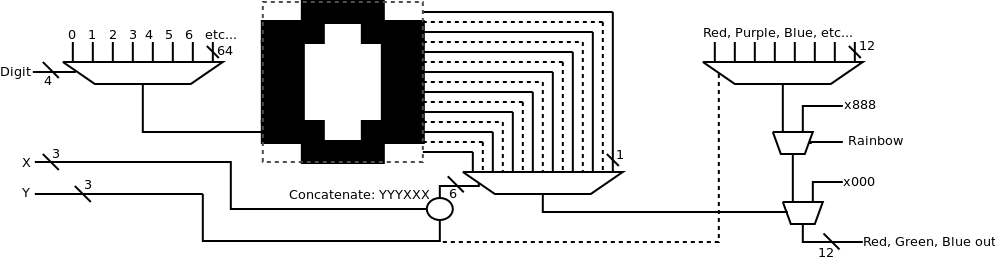
\includegraphics[width=7in]{Digit}
\caption{The dataflow for a pixel of a digit}
\label{Digit}
\end{figure*}

The digits and bricks used convenient size factors to simplify the logic behind rendering. Below is some example code for each:

Digits:
\begin{tabbing}
1.if(\=y $<$\= SC\=REE\=N\_Y\_BEGIN) then\\
2.\>    if(x $<$ 64) then\\
3.\>\>      number $<=$ score(11 downto 8);\\			
4.\>\>		R $<=$ rSymbol;\\
5.\>\>		G $<=$ gSymbol;\\
6.\>\>		B $<=$ bSymbol;\\
7.\>	elsif (x $<$ 128) then\\
8.\>\>		number $<=$ score(7 downto 4);\\
9.\>\>		R $<=$ rSymbol;\\
10.\>\>		G $<=$ gSymbol;\\
11.\>\>		B $<=$ bSymbol;\\
12.\>\>\>$\cdots$\\
13.xSymbol $<=$ std\_logic\_vector(x(5 downto 3));\\
14.ySymbol $<=$ std\_logic\_vector(y(5 downto 3));\\
\end{tabbing}

Bricks:
\begin{tabbing}
15.els\=if(\=(SC\=REE\=N\_BRICK\_BEGIN $<=$ y) and \\
\>\>(y $<$ SCREEN\_BRICK\_END)) then\\
16.\>	vx := std\_logic\_vector(x - SCREEN\_X\_BEGIN);\\
17.\>	vy := std\_logic\_vector(y - SCREEN\_BRICK\_BEGIN);\\
18.\>	vx := ``00000" \& vx(11 downto 5);\\
19.\>	vy := ``000" \& vy(11 downto 3);\\
20.\>	if(bricks(to\_integer(unsigned(vy) $* 18 +$ \\
\>\>\>unsigned(vx))) $= `1' $) then\\
21.\>\> $\cdots$ \emph{Set R,G,B to a colored brick pixel}\\
\end{tabbing}

For the digit code, the digit module in Figure~\ref{Digit} takes xSymbol and ySymbol vectors as an input and outputs rSymbol, gSymbol, and bSymbol vectors. Thus when we have a pixel in the area of a digit we set the outgoing R, G, and B signals to the rSymbol, gSymbol, and bSymbol vectors (lines 4-6 and 9-11). Notice that xSymbol and ySymbol (lines 13 and 14) take bits from the middle of the x and y vectors, dividing the coordinate space by $8 \hbox{ mod } 8$. This makes $8 \times 8$ pixels the same color for a given digit pixel, creating a retro-looking number on the screen.

The bricks used a similar trick for rendering. If the x and y coordinate is within the brick range (line 15), we divide by shifting the x and y coordinate ($8$ for height and $32$ for width, lines 18 and 19). Then by multiplying the y value by the width of the bricks (see Figure~\ref{Screen}), we can index the bricks bit array to see if the brick exists, $1$, or is gone, $0$. To color the bricks we use a multiplexer on the vy value to determine what line a brick is on.

\subsection{Sync}

The Sync is a general purpose module for rastering pixels on a $640 \times 480$ pixel screen at $25$ mhz. Figure~\ref{Sync} shows the counters (A.) required to implement the VGA protocol. These counters are the only source of synchronous, behavioral logic relying on memory. Each indexes the screen along the horizontal axis (x) or the vertical axis (y).

\begin{figure*}[!t]
\centering
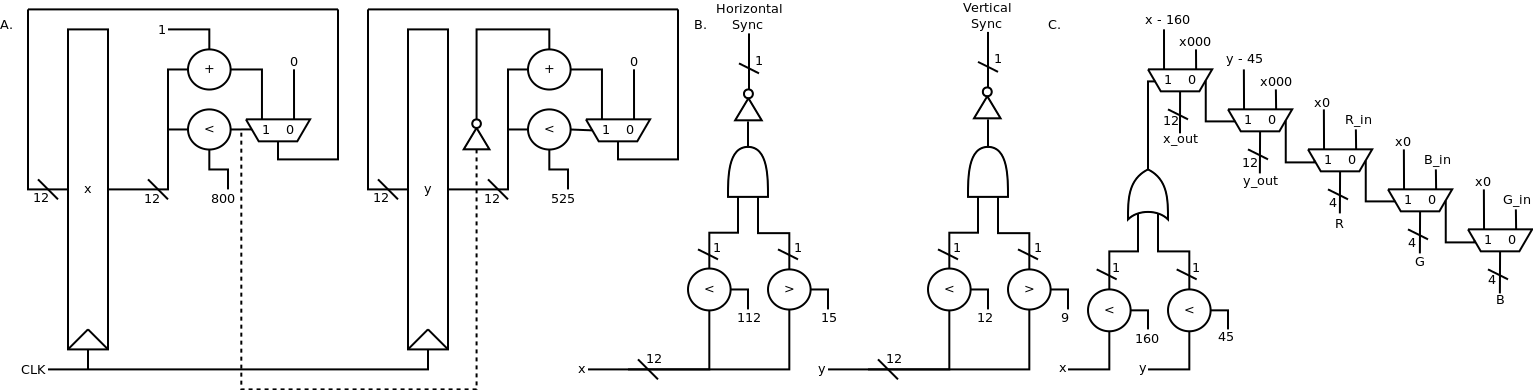
\includegraphics[width=7in]{Sync}
\caption{The sync counters and corresponding dataflow logic}
\label{Sync}
\end{figure*}

The rest of the logic found within the sync relies on dataflow to implement the protocol for a $640 \times 480$ pixel screen. Note that a DCM created by the ISE Xilinx Wizard was required to generate a consistent 25 mhz clock from the board's default 50mhz to drive the index of the screen. Given these conditions, the Sync compares values from the counters with the numbers for the front porch, sync pulse, and back porch. Before the rendering of the screens pixels, the VGA output toggles the sync pulse to off in the middle of the front and back porches. During the front porch, sync pulse, and back porch we keep the R, G and B signals low. After the back porch, we can send the x and y signals out and forward any received R, G, and B colors to the VGA output. Since this module only send out x and y coordinates and colors without any rendering, it can be used in tandem with any hardware component. The x and y coordinates are hooked up to the x and y inputs of BreakRaster, while the R, G, and B outputs are forwarded from the R, G, and B outputs of BreakRaster. If we needed to make a new game, we would likely have to switch out BreakRaster; however, the Sync module would stay exactly the same.

\section{Game Logic}

\subsection{Inputs and Outputs}

\begin{figure*}[!t]
\centering
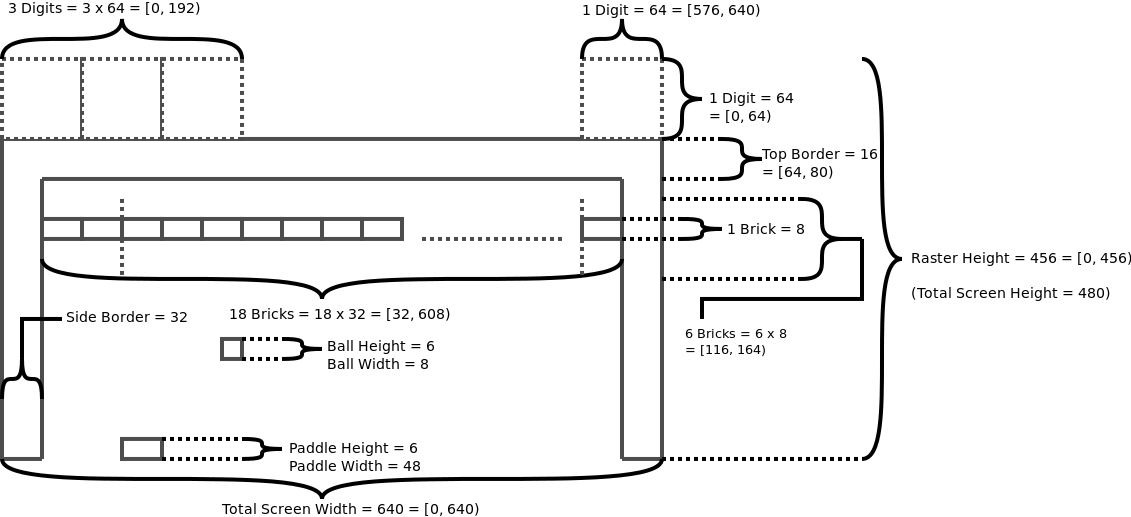
\includegraphics[width=7in]{Screen}
\caption{The specifications for the screen}
\label{Screen}
\end{figure*}

Much of the game logic depends on the specifications for the screen in Figure~\ref{Screen} examined in the previous section. We  parameterized collisions with bricks, the paddle, and the size of the ball using these specification for ease of editing later in the process. The game logic module required signals for the clock and reset as well as signals from the keyboard controller: control\_en, control\_mode, control\_signal.

All of the outputs feed into the VGA controller: paddle\_x, ball\_x, ball\_y, bricks, lives, score, dead, and draw\_mode. The dead signal was used in

In addition to the input and output signals, game logic featured several internal registers including:
\begin{itemize}
  \item ball\_x\_dir: The horizontal direction of the ball, `1' for right and `0' for left.
  \item ball\_y\_dir: The vertical direction of the ball, `1' for up and `0' for down.
  \item paddle\_x\_dir: The direction of the paddle, `1' for right and `0' for left.
  \item paddle\_moving: An enable signal for whether the paddle should move.
  \item angle\_reg: A register for the angle of the ball (i.e. low, med, and hi).
  \item speed\_reg: A register for the speed of the ball (e.g. slow, normal, fast, etc.)
  \item clk50MhzCounter: A counter for the number of 50mhz cycles from the input clock.
  \item clk50hz: A ``slow" clock for the updates of the game logic.
\end{itemize}

\begin{figure}[!t]
\centering
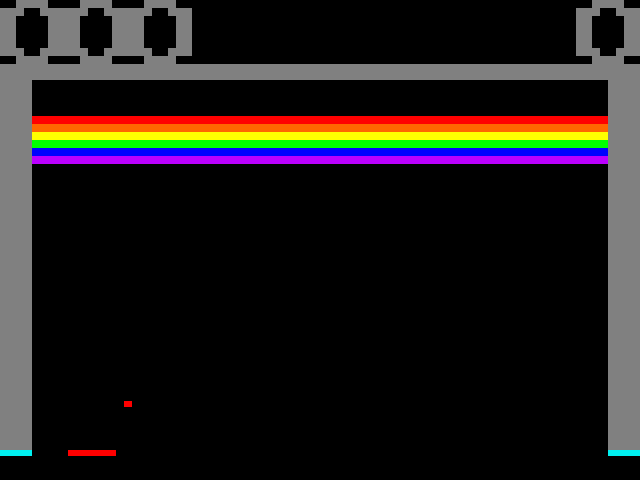
\includegraphics[width=3.5in]{ActualScreen}
\caption{The screen as implemented on the FPGA}
\label{ActualScreen}
\end{figure}

Figure~\ref{ActualScreen} shows how the screen looks when rendered on the screen.


\subsection{Speed and Points}


\subsection{Collisions}
Collisions between the ball with the side walls and the paddle were done using conditional comparators such as $<$ or $>=$. Based off of the specifications of the screen, the ball would check if its location was out of the drawn boundaries. If so, it would adjust its position (either the ball\_x or ball\_y signals) accordingly and bounce by switching its horizontal or vertical direction. In the cases where the ball left the bounds of the bottom of the screen without colliding with the paddle, the player would lose a life.


\section{For the Future}
\subsection{Open Issues}
One issue comes from increasing the speed of the ball. At the top speed, the ball sometimes skips over bricks. In a conventional processor this problem could elegantly be solved by some code; however, the quest for an equally elegant hardware solution has so far confounded the authors of this paper. However, there may also exist many clumsier ``brute force" solutions that would be easier to implement, albeit a waste of reconfigurable logic.
\subsection{Lessons Learned}
As the project winded down the quality of the code reflected the energy of the authors. Though the code works, it has a bit of a tired, lazy feel to it, lacking comments or optimal clarity. For a tutorial the code may need some refactoring. The effort required to write code presentable to a learner of VHDL easily outweighs the effort of designing a working piece of hardware. More code reviews and ongoing, consistent commenting may help for future projects.
\subsection{Plans for the Future}
I(Brian) will probably finish a tutorial for this and post it on my web site. Thinking of this from a teaching perspective creates much needed experience for developing curriculums in addition to being a cute resume builder.
\section{Conclusion}
We have accomplished what we set out to do in our proposal to a satisfactory level.



\end{document}


